\chapter{Related Work}
For better understanding of the portfolio selection problem and particle swarm optimisation, their strengths, weaknesses and applications, a study of previous and related works for the measure of risk in a portfolio and alternatives to PSO was made. I will read and evaluate some strengths and weaknesses on the related models and outline where they fail when compared to what this project wants to achieve. 

  \section{Markowitz Model} % (fold)
  \label{sec:markowitz_model}
    One of the first contributions to the portfolio problem was made by Markowitz \cite{marko1} which was later described in more detail in his book \cite{marko2}. Markowitz introduced the mean-variance model which considers the variance of the portfolio as the measure of the investor's risk under a set of assumptions. According to Markowitz, the portfolio selection problem can be expressed as an objective function subject to linear constraints. 

    Following Markowitz, the investment horizon includes a single period whereas the investment strategy is to select an optimal portfolio at the beginning of the period which will be held unchanged until the date of termination. The joint distribution of one-period security returns is assumed to be a multivariate normal distribution, which in turn follows that the distribution of the portfolio return is also normal. 

    Let $S = (S_1,S_2,S_3, \dots , S_N)$ be the set of $N$ assets where each asset $S_i$ has a rate of return represented by a variable $R_i$ with an expected return $r_i$ and each pair of assets $(S_i,S_j)$ has a covariance $\sigma_{ij}$ . The variance-covariance matrix $\sigma_{n\times n}$ contains all the covariance values, furthermore, it is a symmetric matrix and every diagonal element $\sigma_{ii}$ represents the variance of asset $S_i$. Let $\pi$ be a positive value which represents the investor's required expected return. Generally the values $r_i$ $\sigma_{ij}$ are estimated from past data and are fixed during the period of investment. 

    According to Markowitz, a portfolio is a real valued vector $X = (x_1,x_2,x_3, \dots ,x_i)$ where each variable $x_i$ represents the percentage invested in a corresponding asset $S_i$. The value $\sum\limits_{i=1}^N \sum\limits_{j=1}^N x_i x_j \sigma_{ij}$ is the variance of the portfolio and it is the measure of risk associated with the portfolio. From this, we may obtain a constrained portfolio optimisation problem: 
    \begin{equation}
      \begin{split}
        \mbox{\textit{Minimise  }} \sum\limits_{i=1}^N \sum\limits_{j=1}^N x_i x_j \sigma_{ij} \\
        \\\\
        \mbox{\textit{Constraints:} }
        \sum\limits_{i=1}^N x_i r_i = \pi \\
        \sum\limits_{i=1}^N x_i = 1 \\
        0 \leq x_i \leq 1, i \in \{1,2,\dots,N\}
      \end{split}
    \end{equation}

    Here, the objective function minimises the total variance (risk) associated with a portfolio whilst the constraints ensure that the portfolio meets the expected required return of $\pi$ and the proportions of all the assets sum to 1. The non-negative constraint means that no short-selling is allowed. 

    This framework presumes that the investor uses a quadratic utility function or that asset returns follow a multivariate normal distribution. This implies that the rate of return of a portfolio of assets can be completely explained by the expected return or variance of assets. The efficient-frontier is the set of assets which provide minimum risk for a specified level of return. Solving the Markowitz portfolio optimisation problems for different specified expected portfolio returns will give us a set which represents the efficient-frontier, it is a smooth semi-increasing curve which represents the best possible trade-off between risk and expected return, also called the set of Pareto-optimal portfolios \cite{pareto}. 

    \begin{figure}[H]
      \centering
        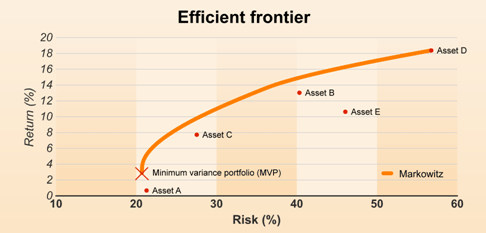
\includegraphics[width=0.9\textwidth]{efficient_frontier}
      \caption{Example of an Efficient Frontier Without a Risk-Free Asset \cite{efficient_frontier}.}
      \label{efficient_frontier}
    \end{figure}

    Each point on the line in Figure~\ref{efficient_frontier} represents a portfolio which is considered to be efficient (ie no other portfolio provides higher return without more risk and similarly for risk). In Figure~\ref{efficient_frontier} Assets A-E represent what the portfolio will be made out of. 

    Markowitz's model is subject to serious criticisms as stated in \cite{crit}, and the main ones being that a measure of dispersion can be adopted as a measure of risk only if the relevant distribution is symmetric. Another problem is that the distribution of individual asset returns has a tendency to show a higher probability of being fat-tailed. In case of non-normal, non-symmetric distributions, the utility function must be quadratic \cite{crit}. 

    This criteria should not be taken lightly since the assets' return does not follow normal distributions in real world situations \cite{non-dist}. This approach can only be used if the investor's utility function is quadratic with non-positive second derivatives or if the asset's return distribution can be fully described. Several research have indicated that that the quadratic utility function implies that beyond some level or return, marginal utility of the decision maker for wealth becomes negative \cite{crit2,crit3}. 
  % section markowitz_model (end)

  \section{Hill Climbing} % (fold)
  \label{sec:hill_climbing}
  Hill climbing \cite{hill,hill2} is an iterative optimisation algorithm which belongs to the family of local search. The algorithm must begin with an arbitrary solution to a problem, then attempts to find a better solution by incrementally changing single elements of the solution. It repeatedly iterates through new solution until no further improvements can be found. 

  The following pseudo-code is a basic hill climbing algorithm:

    \begin{algorithm}[H] \label{eq:hill}
      currentNode = startNode; \\
      \While{not endingCondition()}{
        L = NEIGHBORS(currentNode) \\
        nextEval = -INF \\
        nextNode = NULL \\
        \For{all x $\in$ L}{
          \If{EVAL(x) $>$ nextEval}{
            nextNode = x \\
            nextEval = EVAL(x) \\
          }
        }
        \If{nextEval $\leq$ EVAL(currentNode)}{return currentNode}
        currentNode = nextNode
      }
      \caption{Discrete Space Hill Climbing pseudo-code.}
    \end{algorithm}
  When local search algorithms, such as hill climbing, come across functions, such as $f(x)=\sum\limits_{i=1}^n -x_i sin(\sqrt{|x_i|})$ which was considered \cite{localmin} as a particularly hard function to optimise due to the number of local minima increases exponentially with the number of dimensions of the searching space, they very quickly and easily get trapped in a local optima. This is absolutely not acceptable, specially when there are hundreds of thousands of pounds at stake. 

  There are some improved hill climbing implementations \cite{hill3} where they force more randomness into the algorithm making it behave more like a genetic algorithm. The possibility of becoming stuck in a local optimal instead of the global is the biggest reason why I would choose PSO and other evolutionary algorithms over hill climbing. 

  Scalability is another major factor when considering an optimisation algorithm. Hill climbing will just not be able to cope with the amount of dimensions that the portfolio optimisation function belongs to. These are the biggest reasons why I have chosen not to use Hill climbing or similar local search algorithms. 

  % section hill_climbing (end)

  % \section{Alternative Optimisation} % (fold)
  % \label{sec:alternative_optimisation}
  %   Some other optimisation like simplex method or hopefully something better which is not as good at solving the portfolio optimisation problem as PSO is. 
  %   Hill climbing / greedy search - simplex - scalability problem on deterministic. Easy for hill climbing to get stuck in local opt
  % % section alternative_optimisation (end)

  %------------------------------------------------------------------
  % \section{Heuristic and Metaheuristic Algorithms} % (fold)
  % \label{sec:heuristic_and_metaheuristic_algorithms}
  %   The use of heuristics is very attractive to solve real world problems. For many problems, a heuristic algorithm may be the unique way to obtain good solutions in a reasonably short space of time. Meta-heuristics, a subfield of general heuristic strategies, includes stochastic components to utilize randomised search capabilities. 

  %   In real world applications, 

  % % section heuristic_and_metaheuristic_algorithms (end)
  %------------------------------------------------------------------

  % \section{Portfolio in Excel} % (fold)
  % \label{sec:portfolio_in_excel}
    
  % % section portfolio_in_excel (end)

  % \section{Something PSO} % (fold)
  % \label{sec:something_pso}
  
  % % section something_pso (end)

  % \section{PSO applied} % (fold)
  % \label{sec:pso_applied}
  
  % % section pso_applied (end)

